\documentclass[a4paper,12pt,french]{article}
\usepackage[T1]{fontenc}
\usepackage[utf8]{inputenc}
\usepackage{graphicx}
\usepackage{calc}

\usepackage[french]{babel}

\usepackage[version=4]{mhchem}
\usepackage{siunitx}
\usepackage{amssymb}

\newcommand{\e}[1]{\vspace{5mm}\noindent \textbf{\underline{#1}}}

\newcommand{\makeline}{\noindent\makebox[\linewidth]{\rule{\linewidth}{0.4pt}}} 

\setcounter{secnumdepth}{-1}

\begin{document}

\section{Exercice 1}

Dans certaines piles à combustibles, on utilise le dihydrogène gazeux comme combustible et le dioxygène gazeux comme comburant. La réaction ne produit que de l'eau liquide.

\begin{enumerate}
	\item \label{question1} Écrire l'équation modélisant la réaction avec le coefficient stœchiométrique du dihydrogène égal à $1$.
	
	Cette réaction est en fait l'association de deux demi-équations d'oxydoréduction mettant en jeu les couples oxydant-réducteur \ce{H+_{(aq)}/H2_{(g)}} et \ce{O2_{(g)}/H2O_{(l)}}.
	
	\item Écrire les deux demi-équations d'oxydoréduction et montrer qu'elles permettent effectivement d'obtenir la réaction de combustion trouvée en \ref{question1}.
	\item Les deux demi-réactions ont lieu sur deux électrodes. Indiquer la réaction cathodique et la réaction anodique.
	\item Donner l'expression du potentiel d'oxydoréduction pour les deux couples (à $\SI{298}{\kelvin}$).
	\item Exprimer la constante d'équilibre $K^\circ$ en fonction des potentiels standards des couples en présence. Calculer sa valeur et commenter.
\end{enumerate}

\newpage

\section{Exercice 2}

Deux plaques cylindriques parallèles d'axes $(O_1, z)$ et $(O_2, z)$ de même rayon $a$ sont distantes de $2D = O_1O_2$. Un point $M$ du plan contenant les deux axes, et situé entre les deux cylindres est repéré par ses coordonnées $M(x, z)$, l'origine $O$ du repère étant le milieu de $[O_1O_2]$.

\begin{figure}[h]
	\centering
	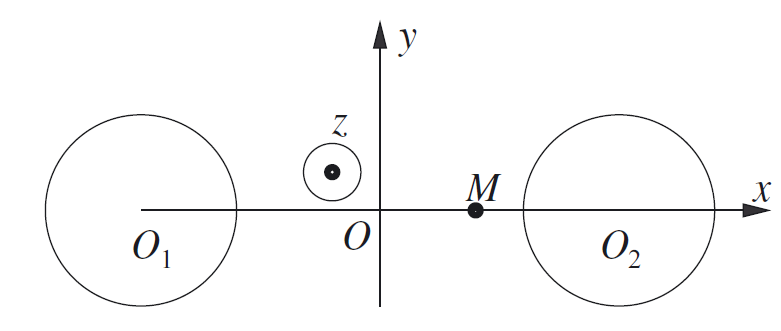
\includegraphics[width = .7\textwidth]{ex_02.png}
\end{figure}

\begin{enumerate}
	\item Considérons pour commencer un cylindre infini d'axe $z$ et de rayon $a$, portant une densité surfacique de charge uniforme $\sigma$. Déterminer le potentiel électrique $V(r)$ en un point quelconque situé à une distance $r$ de son axe.
	\item Le cylindre $1$ du dispositif porte une densité de charge surfacique uniforme $\sigma$, le $2$ une densité $-\sigma$. Dessiner quelques lignes de champ électrique. Faire également figurer quelques équipotentielles.
	\item Déterminer le potentiel électrique $V(x)$ en $M$.
	\item En déduire la tension électrique $u$ entre les deux plaques.
	\item Rappeler l'expression de la capacité électrique d'un condensateur de charge $Q$ et tension $U$.
	\item En déduire l'expression de la capacité $C_H$ d'un tronçon de longueur $H$ du dispositif puis exprimer la capacité linéique $\Gamma = C_H/H$. Commenter le cas limite $a \approx D$.
\end{enumerate}

\newpage

\begin{scriptsize}
	
\e{Nom :} \hfill \e{Date :} \hspace{3cm}

\begin{center}
\begin{tabular}{|p{.1\textwidth}|p{.8\textwidth}|p{.1\textwidth}|}
	\hline
	& \textbf{Ex 1 : Compréhension et application du cours (3 points)} & \\ \hline
	0/3 & Notions mal connues ou mélangées. Définitions, lois ou relations fondamentales non sues ou mal énoncées. & \\ \hline
	1/3 & Cours globalement su mais difficultés à l'appliquer ou trop d'imprécisions dans les énoncés. & \\ \hline
	2/3 & Cours plutôt bien énoncé et appliqué mais quelques imprécisions sur des points classiques. & \\ \hline
	3/3 & Cours connu, énoncé avec précision et appliqué avec rigueur. & \\ \hline
	& \textbf{Ex 2 : Compréhension et application du cours (3 points)} & \\ \hline
	0/3 & Notions mal connues ou mélangées. Définitions, lois ou relations fondamentales non sues ou mal énoncées. & \\ \hline
	1/3 & Cours globalement su mais difficultés à l'appliquer ou trop d'imprécisions dans les énoncés. & \\ \hline
	2/3 & Cours plutôt bien énoncé et appliqué mais quelques imprécisions sur des points classiques. & \\ \hline
	3/3 & Cours connu, énoncé avec précision et appliqué avec rigueur. & \\ \hline
	
	& \textbf{Calculs littéraux et numériques (3 points)} & \\ \hline
	0/3 & Trop d'erreurs de calcul ou d'applications numériques. & \\ \hline
	1/3 & Encore trop d'erreurs. & \\ \hline
	2/3 & Quelques erreurs ou justifications peu convaincantes dans les calculs. & \\ \hline
	3/3 & Calculs bien menés ou corrigés en autonomie. & \\ \hline
	
	& \textbf{Démarche scientifique (3 points)} & \\ \hline
	0/3 & Démarche désorganisée, sans stratégie apparente ou incohérente avec l'énoncé. & \\ \hline
	1/3 & Tentative de stratégie mais manquant de rigueur ou mal adaptée au problème. & \\ \hline
	2/3 & Démarche globalement logique et structurée mais quelques étapes floues ou peu justifiées. & \\ \hline
	3/3 & Démarche claire, logique et rigoureuse. & \\ \hline
	
	& \textbf{Esprit critique et vérification des résultats (2 points)} & \\ \hline
	0/2 & Les résultats ne sont pas critiqués a posteriori & \\ \hline
	1/2 & Démarche critique mais quelques erreurs non corrigées ou interprétations de certains résultats peu convaincantes. & \\ \hline
	2/2 & Utilisation systématique de l'homogénéité, de l'interprétation physique ou de la comparaison à des expressions ou des ordres de grandeur connus, permettant de corriger certaines erreurs en autonomie ou d'apporter un éclaircissement scientifique. & \\ \hline
	
	& \textbf{Expression orale (2 points)} & \\ \hline
	0/2 & Expression confuse, vocabulaire inadapté, fautes répétées d'expression. & \\ \hline
	1/2 & Expression compréhensible mais parfois imprécise ou peu fluide & \\ \hline
	2/2 & Expression claire, structurée et précise. Vocabulaire scientifique. & \\ \hline
	
	& \textbf{Expression écrite (2 points)} & \\ \hline
	0/2 & Tableau mal tenu, absence de figures, notations incorrectes ou dessins inutilisables. & \\ \hline
	1/2 & Tableau soigné mais les schémas manquent de lisibilité ou de pertinence. & \\ \hline
	2/2 & Tableau soigné. Schémas clairs, bien annotés, exploités dans l'argumentation. & \\ \hline
	
	& \textbf{Réactivité aux questions et indications (1 point)} & \\ \hline
	0/1 & Incapacité à comprendre les questions ou à s'adapter aux remarques. & \\ \hline
	1/1 & Bonne écoute, réponses adaptées et correction rapide d'éventuelles erreurs. & \\ \hline
	
	& \textbf{Autonomie et initiative (1 point)} & \\ \hline
	0/1 & Attend des indications pour avancer. & \\ \hline
	1/1 & Prend des initiatives réfléchies, explore différentes pistes avec jugement. & \\ \hline
	
	& \textbf{Total (20 points)} & \\
	& & \\ \hline
\end{tabular} 
\end{center}
\end{scriptsize}

\end{document}